\section{Algoritme til detektering af gang og løb}\label{sec:algogangloeb}
\textit{Dette afsnit omhandler design, implementering og test af algoritmerne til detektering af aktiviteterne gang og løb. Først designes algoritmen til detektion af henholdsvis gang og løb, hvorefter denne implementeres. Afslutningsvist bliver algoritmen testet i forhold til de opstillede krav i \secref{krav_algoritme}.} 
%bliver design af algoritmerne behandlet, hvilket er ensbetydende med at implementering og kodning kan foregå. Når algoritmerne er designet og implementeret bliver de efterfølgende testet for at af- eller bekræfte deres virkning.}

For at kunne adskille gang og løb benyttes et accelerometer, som er beskrevet i \secref{sec_design_LSM9DS1}. For at kunne detektere og adskille disse aktiviteter behandles inputtet fra sensoren gennem forskellig signalbehandlingsprocessor. Algoritmerne gør det muligt at afgøre, om de pågældende signaler repræsenterer gang, løb eller ingen fysisk aktivitet. 

\subsubsection{Design} \label{design_algo_g_l}
Algoritmen som skal detektere gang eller løb designes til at benytte accelerometerets data, med henhold til \appref{pilot}. Dette design fremgår som flowchart på \figref{fig:design_algoritme_gang_loeb}.
\begin{figure}[H]
	\centering
	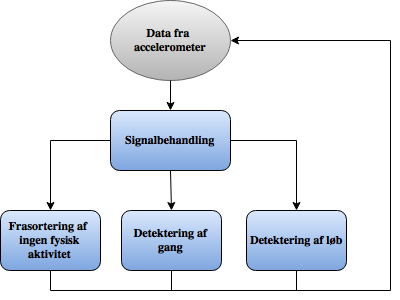
\includegraphics[scale=0.7]{figures/cDesign/design_algoritme_gang_loeb.png}
	\caption{På figuren ses et flowchart over algoritmen til detektering af ingen fysisk aktivitet, gang og løb.}
	\label{fig:design_algoritme_gang_loeb}
\end{figure}
Algoritmen skal benyttes accelerometerets data til at detektere hvorvidt brugeren ikke udfører fysisk aktivitet, går eller løber. \\
Førend denne detektering, skal accelerometeres data signalbehandles for afslutningsvis at kunne benytte tærkselværdier til at detektere hvilken aktivitet der udføres. Signalbehandlingen indebærer filtrering, dividering, kvadrering og moving average filtrering. Denne type signalbehandling af illustreret på \figref{fig:algoritme_behandling}.
\begin{figure}[H]
	\centering
	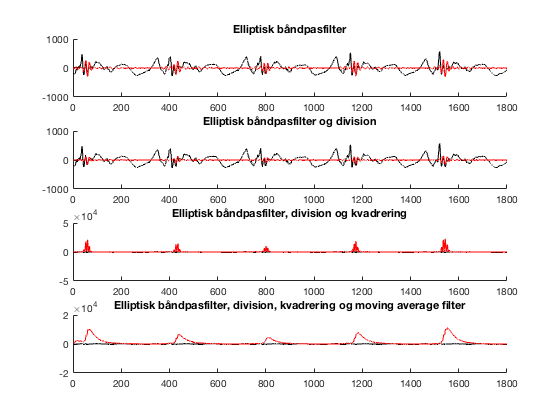
\includegraphics[width=1\textwidth]{figures/cDesign/signalbehandling_psoc.png}
	\caption{På figuren ses de fire signalbehandlingsfunktioners effekt på rå data fra accelerometeret under løb. Den sorte kurve på de fire figurer er det rå signal, og den røde er det behandlede output. Der gøres opmærksom på, at y-aksen ikke er ens for henholdsvis de to øvre og de to nedre figurer, hvorfor det sorte, rå signal bliver en næsten lige linje på de to nedre figurer.}
	\label{fig:algoritme_behandling}
\end{figure}
Signalbehandlingen har til formål at tydeliggøre hælnedslag, for derefter at kunne implementere tærskelværdier til adskillelse af de fysisk aktiviteter. \\
Første del af signalbehandlingen er en filtrering med et elliptisk båndpassfilter, som benyttes til at dæmpe støj. Dette skal være et fjerde ordens elliptisk båndpasfilter med et pasbånd fra 20~Hz til 50~Hz, og med en dæmpning på 60~dB\fxnote{og 0.5 dB peak-to-peak ripples - frekvenserne for gang og løb lå mellem 25 og 45}. Båndpasfilterets knækfrekvenser er valgt med hensyn til pilotforsøget i \appref{pilot}, hvorfra det vurderes at hælnedslag har en frekvens på 25~Hz til 45-~Hz. Ved at benytte et båndpass filter bliver det ønskede signal i frekvensområdet 25-45~Hz bevaret, og andre frekvensen dæmpes.\\
Dernæst bliver signalet behandlet ved brug af en division, som har til formål at sænke amplituden af mindre spikes i signalet. Idet hælnedslaget har den største amplitude i signalet, da bliver amplituden for hælnedslaet fortsat større end de mindre spikes, efter divisionen har indtruffet. \\
Efter signalet er blevet divideret, da kvadreres dette for dermed at øge amplituden af de fremtrædende spikes i signalet. Dermed minimeres de mindre spikes kraftigt, som ikke relateres til hælnedslaget, og selve hælnedslaget forstærkes og tydeliggøres. \\
Afslutningsvis filtreres signalet med et moving average filter, som udglatter signalet, hvorved små udslag ikke opfattes, og signalets hælnedslag vil fremstå som et enkelt spike.

Ovenstående signalbehandling giver et signal med peaks, som skal adskilles med tærskelværdier for henholdsvis gang og løb. Førend en værdi for denne tærskelværdi kan fastsættes, skal dataet fra pilotforsøgets omregnes til ICens enhed for outputdata. ICens arbejdsområde er opgivet i bytes, som følge af ICens 16 bits ADC arbejdsområde. Pilotforsøgets data skal derfor omregnes til bytes, idet data fra pilotforsøget er optaget med Shimmer3 som har enheden, $m/s^{2}$. Derfor bliver pilotforsøgets data først omregnet til g, hvorefter denne være omregnes med henhold til opløsningen for den 12 bits ADC som er placeret i Shimmer3. For at gøre dette benyttes accelerometerets sensitivitet, som er 0,012 g/LSB. Data fra shimmer som er omregnet til g, skal divideres med accelerometerets sensitivitet. Outputet fra Shimmer3 og ICen er nu samme enhed, som det fremgår af \eqref{eq:bitsammenhaeng}.
 
\begin{equation}
\frac{32 g \cdot 2^{16}}{32 g \cdot 2^{12}} = 16
\label{eq:bitsammenhaeng}
\end{equation}

Data fra Shimmer3 skal derfor multipliceres med 16, hvilket medfører samme enhed for de to systemer. Det er derefter muligt, at vurdere hvilket tærskelværdier som kan benyttes til at detektere gang og løb.\\
De behandlede signaler fra pilotforsøget, benyttes med henblik på fastsættelse af tærskelværdier. \tabref{tab:individuel_taerskel} viser tærskelværdierne for de fire forsøgspersoner, hvoraf tærskelværdierne er bestemt med henhold til de behandlede signaler. 
\begin{table}[H]
	\centering
	\begin{tabular}{ccc}
		\hline
		\rowcolor[HTML]{C0C0C0} 
		Forsøgsperson & Tærskelværdi for gang & Tærskelværdi for løb \\ \hline
		\rowcolor[HTML]{FFFFFF} 
		F1 & 50 & 1050 \\ \hline
		\rowcolor[HTML]{FFFFFF} 
		F2 & 55 & 500 \\ \hline
		\rowcolor[HTML]{FFFFFF} 
		F3 & 50 & 400 \\ \hline
		\rowcolor[HTML]{FFFFFF} 
		F4 & 150 & 100 \\ \hline
	\end{tabular}
	\caption{I tabellen ses tærskelværdierne for forsøgspersonerne ved aktiviteterne gang og løb.}
	\label{tab:individuel_taerskel}
\end{table}\vspace{-0.5cm}
De individuelle tærskelværdier i \tabref{tab:individuel_taerskel} er fundet over et fem sekunders vindue for hver forsøgsperson. Heraf antages det, at tærskelværdierne er repræsentative for den fysiske aktivitet idet aktiviteten blev udført ved konstant hastighed. Ydermere skal systemet være gældende for en stor population, hvormed en given tærskelværdierne for gang og løb skal være dækkende for alle forsøgspersoner. En samlet tærskelværdi, der er dækkende for samtlige forsøgspersoners data, ses i \tabref{tab:faelles_taerskel}.
\begin{table}[H]
	\centering
	\begin{tabular}{ccc}
		\hline
		\rowcolor[HTML]{C0C0C0} 
		Tærskelværdi for ingen fysisk aktivitet & Tærskelværdi for gang & Tærskelværdi for løb \\ \hline
		x \textless~50 & 50 \textless~x~\textless 400 & x~$\geq$~400 \\ \hline
	\end{tabular}
	\caption{I tabellen ses de tærskelværdier, som for alle forsøgspersoner vil kunne detektere og adskille gang og løb fra hinanden.}
	\label{tab:faelles_taerskel}
\end{table}\vspace{-0.5cm}
Fastsættelsen af den fælles tærskelværdi bør sikre, at gang og løb er mulige at detektere samt adskille for forsøgspersonernes data. Igennem behandling af data fra pilotforsøget forekom tærskelværdierne i \tabref{tab:faelles_taerskel} dækkende for alle forsøgspersonerne, hvorfor disse blev valgt.

\subsection{Implementering}
Implementeringen af algoritmen for detektering af gang og løb tager udgangspunkt i data fra pilotforsøget og de designmæssige aspekter, som er beskrevet i \secref{design_algo_g_l}. Algoritmen er designet og implementeret, som det ses på \figref{fig:basic_algo_g_l}.
\begin{figure}[H]
	\centering
	\includegraphics[scale=0.6]{figures/cDesign/Algoritme_g_l_basic.png}
	\caption{På figuren ses den overordnede C kode for algoritmen til detektering af gang og løb beskrevet med pesudokode. De markerede kasser vil blive forklaret yderligere i kommende figurer.}
	\label{fig:basic_algo_g_l}
\end{figure} \vspace{-0.5cm}
Algoritmen henter low og high byte fra ICens outputdata, hvorefter de enkelte samples gennemgår en signalbehandling. Denne signalbehandling og den tilhørende C kode vil blive yderligere forklaret i \figref{fig:signalbehandling_g_l}. Efter samples er blevet behandlet, bliver time\_counteren startet således, at denne tæller antallet af samples mellem bestemte if lykker i algoritmen. De behandlede samples gemmes i variabel Value[0], hvortil den foregående behandlede sample bliver gemt i variabel Value[1]. På denne måde, hvorpå en gammel og ny sample gemmes i hver sin variabel, muliggøres blandt andet, at algoritmen kan undersøge disse variabler i forhold til hinanden og deres størrelse i forhold til en tærskelværdi. \\
Efter den nye og foregående sample er placeret i separate variabler er det muligt at benytte tærskelværdier til at detektere, hvorvidt der er ingen aktivitet, gang eller løb. Disse elementer af algoritmen forklares yderligere i \figref{fig:ingen_ak_pseudo}, \figref{fig:gang_pseudo} og \figref{fig:loeb_pseudo}. Tærskelværdierne for de pågældende fysiske aktiviteter er bestemt i \secref{design_algo_g_l}. \\ 
Yderligere bliver den maksimale peak bestemt, da denne værdi initialiserer, om det er gang eller løb i GUIen. Dette gøres ved at sammenligne, om den forrige sample er større end den nuværende. Hvis dette er tilfældet, betegnes den forrige værende som værende maks peak værdien. %Når kurven derimod er faldende, vil detektering af maksimale peak ikke udføres.

Algoritmens signalbehandling involverer fire elementer; elliptisk filtrering, dividering, kvadrering og en moving average filtrering. Dette ses på \figref{fig:signalbehandling_g_l}.
\begin{figure}[H]
	\centering
	\includegraphics[scale=0.6]{figures/cDesign/Signalbehandling_gl_pesudo.png}
	\caption{På figuren ses algoritmens signalbehandling i C kode beskrevet som pseudokode.}
	\label{fig:signalbehandling_g_l}
\end{figure} \vspace{-0.5cm}
Efter datamodtagelse fra ICen bliver samples IIR filtreret ved hjælp af a og b koefficienter for et elliptisk filter. Efterfølgende retureneres de behandlede samples, hvormed disse er klar til næste del af signalbehandlingen. De pågældende a og b koefficienter bestemmes i MATLAB, hvor filterets knækfrekvenser og dæmpning benyttes til at bestemme det elliptiske filters koefficienter. Disse koefficienter skriver i C koden for algoritmen, således filtreringen er med henhold til det ønskede filter designet i MATLAB.\\
De enkelte samples bliver herefter bitskiftet med 5, hvilket svarer til at dividere med 32\fxnote{2 opløftet i 5}. Derudover bliver samples kvadreret ved at gange hver sample med sig selv. Afslutningsvis filtreres samples med et moving average filter, hvilket medfører en blødere kurve, som ses på \figref{fig:algoritme_behandling}.

Algoritmen er designet og implementeret således, at denne kan detektere, hvis brugeren ikke er fysisk aktiv. Denne del af algoritmen fremgår af \figref{fig:ingen_ak_pseudo}.
\begin{figure}[H]
	\centering
	\includegraphics[scale=0.6]{figures/cDesign/ingen_aktivitet_gl_pseudo.png}
	\caption{På figuren ses algoritmens metode til at detektere, om brugeren er fysisk aktiv eller ej. Det fremgår, at hvis time\_count er større end tre sekunder sampling, som svarer til 1428 samples, da detekteres brugeren som værende ikke fysisk aktiv.}
	\label{fig:ingen_ak_pseudo}
\end{figure} \vspace{-0.5cm}
Algoritmen detekterer, at brugeren ikke er fysisk aktiv, hvis time counteren opnår et antal samples, som er større end tre sekunders sampling. Hvis dette er tilfældet, bliver de pågældende variabler nulstillet og tæller forfra.

Algoritmen benytter tærskelværdier til at bestemme hvorvidt brugeren går eller løber. \Figref{fig:gang_pseudo} viser algoritmens opbygning med henhold til detektering af gang ved brug af tærskelværdier.
\begin{figure}[H]
	\centering
	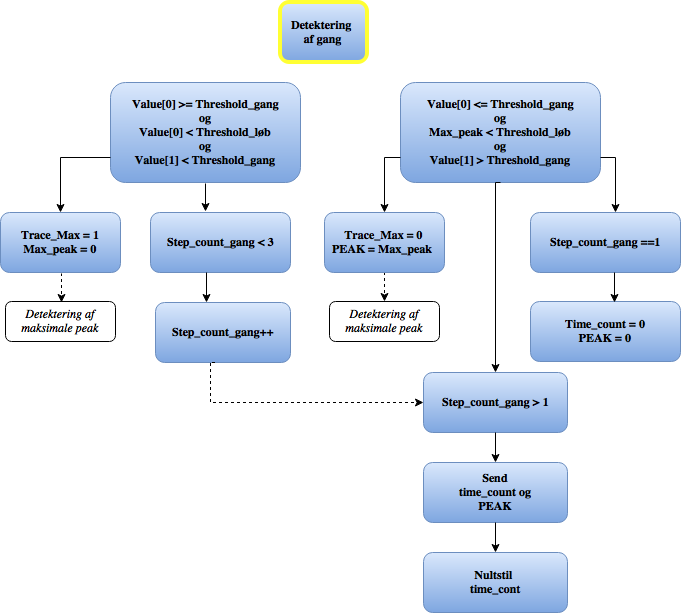
\includegraphics[scale=0.6]{figures/cDesign/gang_ckode_pseudo.png}
	\caption{På figuren ses den implementerede C kode beskrevet med pseudokode. Denne del af algoritmen benyttes til detektering af gang.}
	\label{fig:gang_pseudo}
\end{figure} \vspace{-0.5cm}
Til venstre på figuren ses delen, som er ansvarlig for optælling af skridt, hvortil den højre del visualiserer delen, som bestemmer varigheden mellem hælnedslag ved gang. Førend algoritmen kan tælle op på antal skridt for gang, skal amplituden for Value[0] være i intervallet mellem tærskelværdierne for gang og løb. Yderligere skal den foregående sample Value[1] have en værdi, der er lavere end tærskelværdien for gang. Hvis disse tre kriterier er opfyldt, indstilles Trace\_Max til at være lig 1. Dette tillader, at algoritmen begynder at finde den maksimale peak, som illustreret på \figref{fig:basic_algo_g_l}. Ydermere bliver Step\_count\_gang talt op, indtil denne variabel er maksimalt 3. \\
Højre del af \figref{fig:gang_pseudo} repræsenterer den del af algoritmen, som finder varigheden mellem hælnedslag og sender dette gennem BLE. Førend denne del af algoritmen bliver udført, skal Value[0] være mindre end tærskelværdien for gang og Value[1] skal være over denne tærkselværdi. Yderligere skal det bestemte maksimale peak være mindre end tærskelværdien for løb. Hvis kriterierne opfyldes, bliver det maksimale peak gemt i PEAK, samt algoritmen indstilles således, at denne ikke længere finder et maksimalt peak. Yderligere er det gældende, at hvis der er detekteret ét hælnedslag for gang, bliver henholdsvis time counteren og PEAK nulstillet. \\
For at bestemme varigheden mellem hælnedslag skal antallet af hælnedslag for gang overstige værdien 1. Under disse omstændigheder bliver time\_count og PEAK bitskiftet, hvorefter disse værdier sendes over BLE. Afslutningsvis nulstilles time counteren.

Algoritmen er desuden i stand til at detektere løb, hvilket også gøres ved brug af tærskelværdier, som det ses på \figref{fig:loeb_pseudo}.
\begin{figure}[H]
	\centering
	\includegraphics[scale=0.6]{figures/cDesign/loeb_ckode_pseudo.png}
	\caption{ På figuren ses den implementerede C kode beskrevet med pseudokode. Denne del af algoritmen benyttes til detektering af løb.}
	\label{fig:loeb_pseudo}
\end{figure} \vspace{-0.5cm}
Den venstre del af figuren er ansvarlig for optælling af skridt, hvortil den højre del bestemmer varigheden mellem hælnedslag ved løb. Førend algoritmen kan tælle op på antal skridt for løb, skal amplituden for Value[0] være større end tærskelværdien for løb. Yderligere skal den foregående sample Value[1] have en størrelse, der er lavere end tærskelværdien for løb. Hvis disse to kriterier er opfyldt, indstilles Trace\_Max til at være lig 1. Dette tillader, at algoritmen begynder at finde den maksimale peak, som illustreret på \figref{fig:basic_algo_g_l}. Ydermere bliver Step\_count\_løb talt op, indtil denne variabel er maksimalt 3. \\
Højre del af \figref{fig:loeb_pseudo} repræsenterer den del af algoritmen, som finder varigheden mellem hælnedslag og sender dette gennem BLE. Førend denne del af algoritmen bliver udført, skal Value[0] være mindre end tærskelværdien for løb, og Value[1] skal være over denne tærskelværdi. Hvis kriteriet opfyldes, bliver det maksimale peak gemt i PEAK, samt algoritmen indstilles således, at denne ikke længere finder et maksimalt peak. Yderligere er det gældende, at hvis der er detekteret ét hælnedslag for løb bliver henholdsvis time counteren og PEAK nulstillet. \\
For at bestemme varigheden mellem hælnedslag  skal antal hælnedslag for løb overstige værdien 1. Under disse omstændigheder bliver time\_count og PEAK bitskiftet, hvorefter disse værdier sendes over BLE. Afslutningsvis nulstilles time counteren.

\subsection{Test}
Testen udføres med henhold til de opstillede krav og tilhørende tilladte afvigelser opstillet i \secref{krav_algoritme}. Kravene beskriver, at algoritmen skal:
\begin{itemize}
	\item Behandle data fra accelerometret, således hælnedslag fremstår som et markant peak.
	\item Være i stand til at detektere gang og løb ved brug af tærskelværdier. Det accepteres ingen afvigelse ved detektering af den pågældende aktivitet.
\end{itemize}
Algoritmens funktioner testes individuelt og samlet. Dette gøres ved at indsende et simuleret signal, hvis funktion er at agerer som gang, løb eller ingen aktivitet. Det simulerede signal er et absolut sinussignal med varierende amplitude. Amplituden for det simulerede signal afgør, hvorvidt signalet bør agerer som gang, løb eller ingen aktivitet. Et sinussignal er valgt, da dette har grundlæggende samme karateristik som et eventuelt gang- eller løbesignal. Der ønskes et ideelt signal, som går over og under tærskelværdierne og derved kan aktivere timeren i algoritmen.

Først testes algoritmens time counter, der giver et udtryk for, om algoritmen detekterer gang korrekt. Der indsendes et absolut sinussignal samplet med 512 Hz, en frekvens på 0,5 Hz og en amplitude på 100. Dette resulterede i tre halvbølger med en amplitude på 100 på 1536 samples. Dette kan ses som den sorte kurve på \figref{fig:testgraf_timecounter}.
\begin{figure}[H]
	\centering
	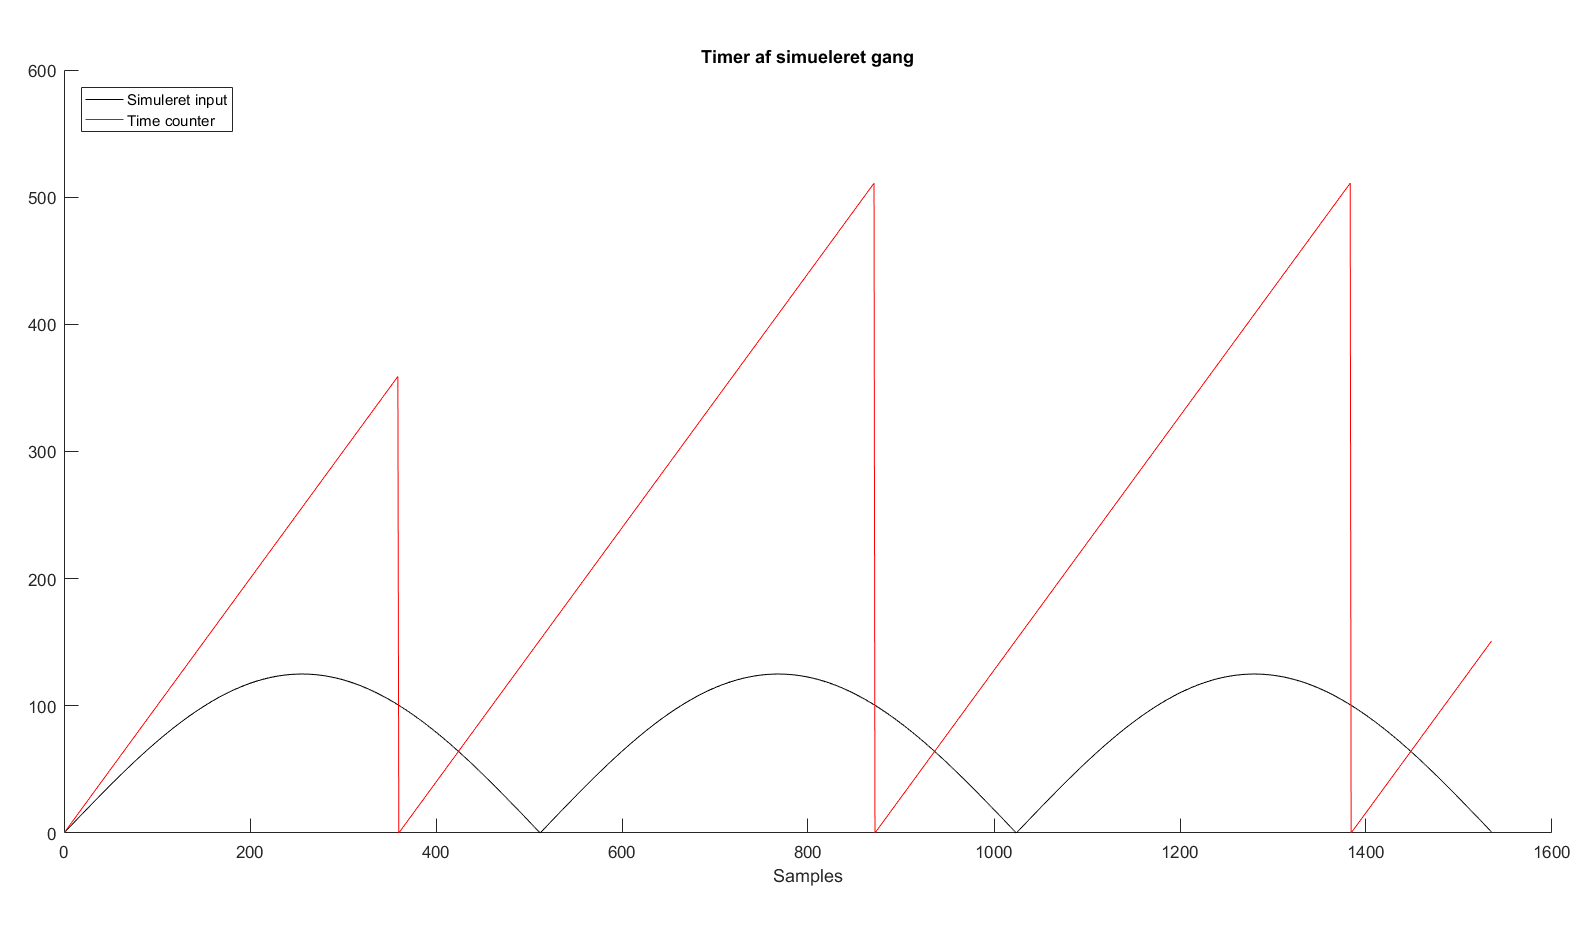
\includegraphics[width=.9\textwidth]{figures/cDesign/test_timecount_gang.png}
	\caption{På figuren ses algoritmens time counter som den røde kurve, der reagerer på detekteringen af et simuleret gangsignal. Denne nulstilles hver gang signalet går under tærskelværdien, således maks peak værdien og tidsværdien sendes videre. Den sorte kurve er det simulerede gangsignal.}
	\label{fig:testgraf_timecounter}
\end{figure}
Algoritmens time counter starter, når signalet bliver indsendt, og nulstilles efter en sample går under tærskelværdien. Heraf kan det ses, at varigheden fra en sample er gået under en tærskelværdi til, at en sample igen er gået under en tærskelværdi er 512 samples. En af algoritmens funktioner er at frasortere det første detekterede peak, dermed nulstille time counter værdien samt peak værdien.\\
Den egentlige test vedrørende algoritmens time counter består dermed i at undersøge, om den første peak tælles med eller ej i videresendt data. I \tabref{tab:test_res_timecount} ses der, at selvom den første peak visualiseres i \figref{fig:testgraf_timecounter}, så medregnet den ikke i de endelige værdier. Disse værdier fås ved hjælp af programmet Realterm, som viser sendt data fra MCUen ved brug af UART.
\begin{table}[H]
	\centering
	\begin{tabular}{ccc}
		\hline
		\rowcolor[HTML]{C0C0C0} 
		Værdi videresendt & Forventet værdi [samples] & Modtaget værdi [samples] \\ \hline
		Time counter & $\emptyset$ - 512 - 512 & $\emptyset$ - 512 - 512 \\ \hline
	\end{tabular}
	\caption{I tabellen ses testresultaterne vedrørende test af time counter. $\emptyset$ antyder at det ikke blev modtaget noget ved første peak.}
	\label{tab:test_res_timecount}
\end{table} \vspace{-0.5cm}
Algoritmen er blevet testet på tre halvbølger, og dermed er det forventede resultat at varigheden af første peak ikke blev medregnet og videresendt som et resultat. Algoritmens time counter fungerede som forventet, og videresendte kun det forventede resultat med præcis nøjagtighed. Denne del af algoritmen accepteres og er klar til implementering i det samlede system.

I anden test af algoritmen tjekkes der for, om algoritmen giver korrekt værdi for maks peak detektering. Denne er designet således, at algoritmen ikke skal registrer det første peak i et signal, som første test beviste ikke sker. På \figref{fig:test_peak_gang} ses resultatet af testen.
\begin{figure}[H]
	\centering
	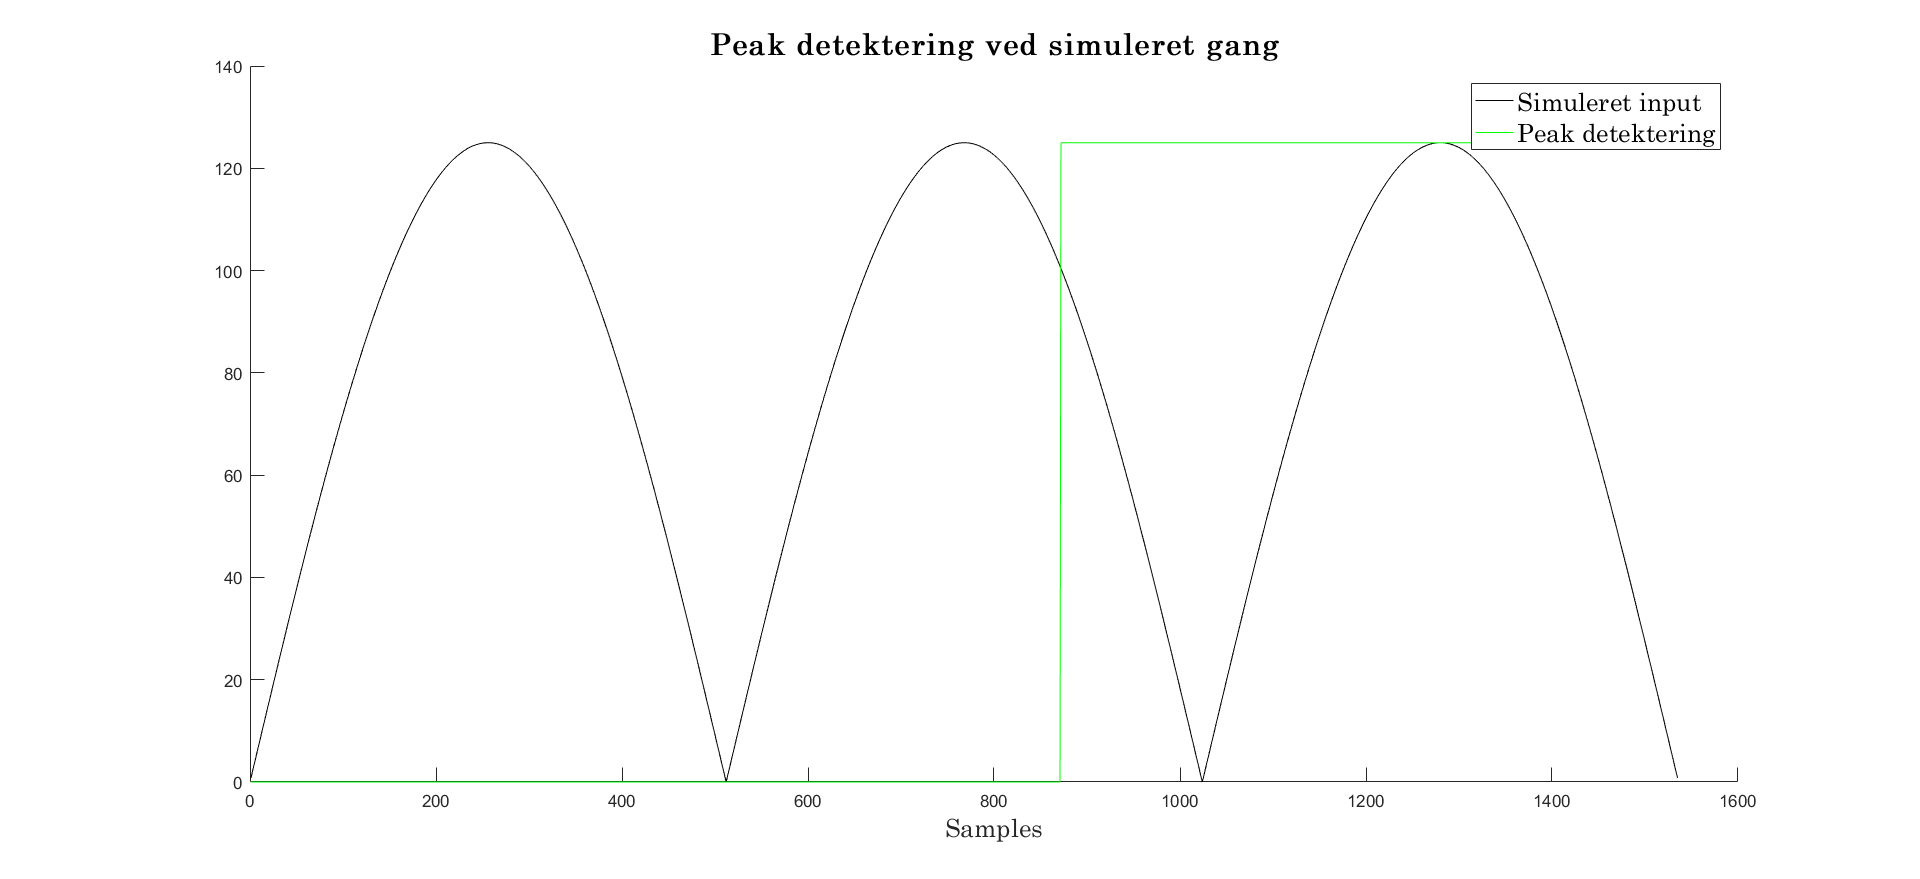
\includegraphics[width=.9\textwidth]{figures/cDesign/test_peak_gang.png}
	\caption{På figuren ses algoritmens funktion til at detektere værdien for maks peak i et simuleres gangsignal. Den sorte kurve er det simulerede gang signal, og den røde kurve viser algoritmens funktion til detektering af peakværdier. Der ses, at den første peak ikke detekteres som ønsket. Herefter findes værdien for det andet maks peak, når signalet er gået under tærskelværdien på 50. Da tredje maks peak har samme værdi som anden maks peak, forbliver den røde kurve på samme værdi.}
	\label{fig:test_peak_gang}
\end{figure}\vspace{-.5cm}
Algoritmens detektering af peak starter, når en sample overskrider en bestemt tærskelværdi, hvilket ikke fremgår tydeligt på \figref{fig:test_peak_gang}. Men algoritmen finder maks peaket, når en sample er under tærskelværdien, hvilket ses ud fra den røde graf. Hvis det første peak detekteres, sættes værdien til nul, således den ikke tælles med. På \figref{fig:test_peak_gang} kan det ses, at når signalet går under tærskelværdien anden gang, bliver peaket registreret. Den egentlige test vedrørende algoritmens detektering af peaks består dermed i at undersøge hvilke data, der videresendes som resultat, efter et input er kørt igennem algoritmen. Resultatet heraf ses i \tabref{tab:test_res_peak}, som fås ved hjælp af programmet Realterm, som viser sendt data fra MCUen ved brug af UART.
\begin{table}[H]
	\centering
	\begin{tabular}{ccc}
		\hline
		\rowcolor[HTML]{C0C0C0} 
		Værdi videresendt & Forventet output [amplitude] & Output [amplitude] \\ \hline
		Peak detektering & $\emptyset$ - 100 - 100 & $\emptyset$ - 100 - 100 \\ \hline
	\end{tabular}
	\caption{I tabellen ses testresultaterne vedrørende test af detektering af peaks. $\emptyset$ antyder at det ikke blev modtaget noget ved første peak. Der ses i tabellen, at outputtet fra testen stemmer overens med det forventede output.}
	\label{tab:test_res_peak}
\end{table}\vspace{-0.5cm}
Algoritmen er blevet testet på tre halvbølger, og dermed er det forventede resultat, at peakværdien af det første peak ikke bliver medregnet og videresendt som et resultat. Algoritmens peak detektering fungerer dermed som forventet og videresendte amplituderne, som halvbølgerne var designet med, med en præcis nøjagtighed. Denne del af algoritmen accepteres og er klar til implementering i det samlede system.

Algoritmen for løb blev ligeledes testet med hensyn til funktionaliteten af time counter og peak detektering. Ved denne test blev der indsendt et absolut sinussignal med en højere amplitude, som ville overskride tærskelværdien vedrørende detektering af løb. Resultaterne af disse test medførte resultater af samme nøjagtighed, som ved detektering af gang. Algoritmen bør dermed fungerer optimalt, både til detektering af gang og løb men testet herunder i samlet plots.

Algoritmen bør altså undersøge, hvorvidt data fra accelerometret klarificeres som ingen aktivitet, gang eller løb ved hjælp af tærskelværdier. I testen heraf indsendes et simuleret signal, som først overskrider tærskelværdierne for gang på 50. Herefter forekommer en periode på tre sekunder, hvor hverken gang eller løbs tærskelværdi overskrides, hvorfor time counteren vil nulstille efter tre sekunder uden overskridelse af nogen tærskelværdier. Afslutningsvis indsendes værdier, som overskrider tærskelværdierne vedrørende løb på 400. Herigennem bliver både time count og detektering af peaks testet, hvilket fremgår i \figref{fig:test_inaktiv_time} og \figref{fig:test_inaktiv_peak}. 
\begin{figure}[H]
	\centering
	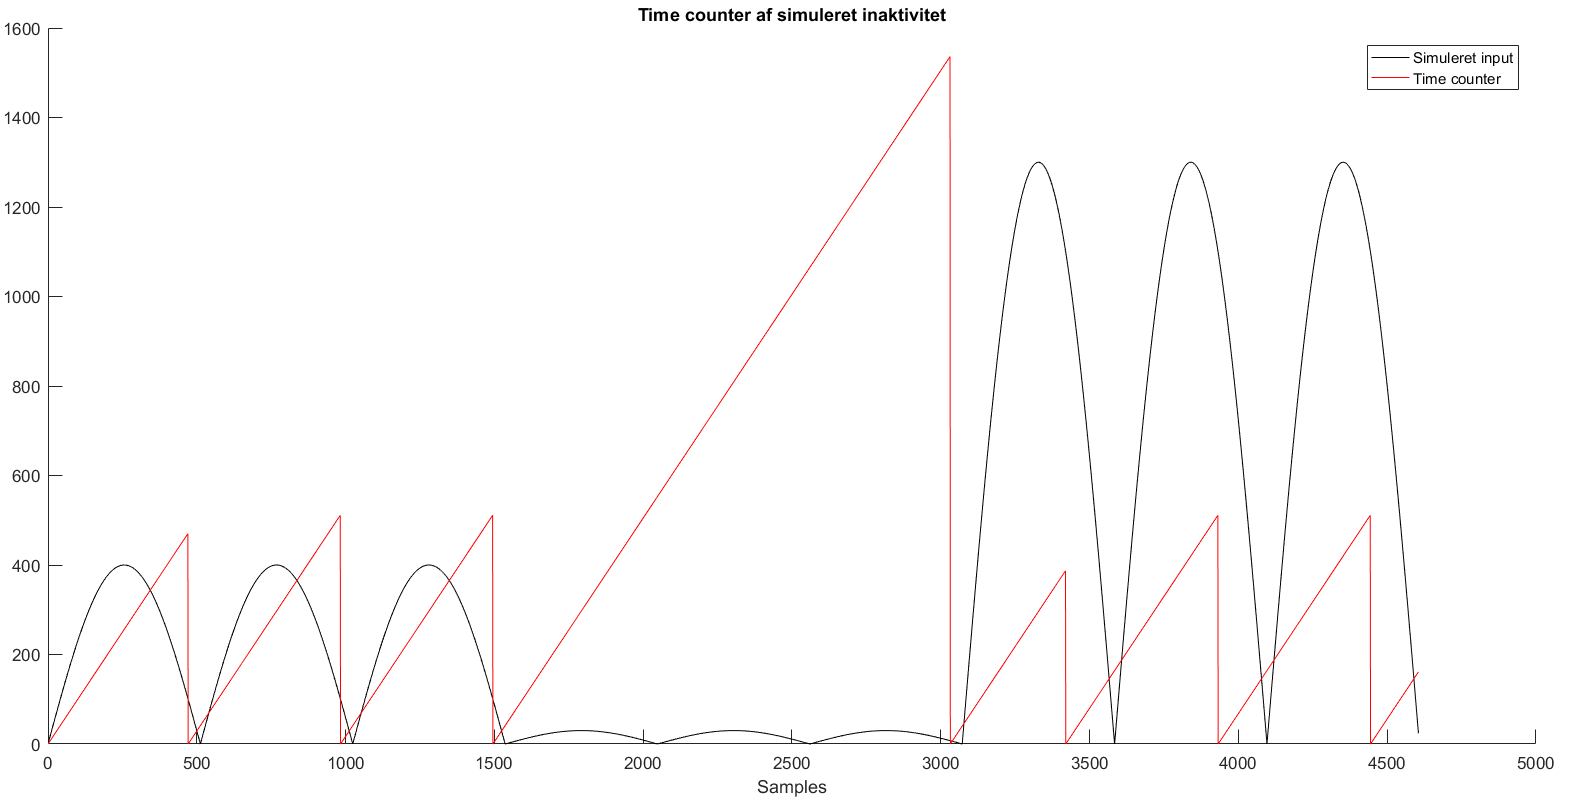
\includegraphics[scale=0.3]{figures/cDesign/test_timecount_inaktiv.png}
	\caption{På figuren ses algoritmens time counter, som resultat af detektering af et simuleret gang, inaktiv og løbe signal. Den sorte kurve er det simulerede signal, og den røde kurve viser algoritmens time counter af samples, som overholder algoritmens specifikationer. Der ses i midten af figuren, at time counteren nulstilles efter tre sekunder selvom inden tærskelværdier er overskredet. Det er derfor fordelagtigt at smide værdien ud for første detekterede maks peak herefter.}
	\label{fig:test_inaktiv_time}
\end{figure}

\begin{figure}[H]
	\centering
	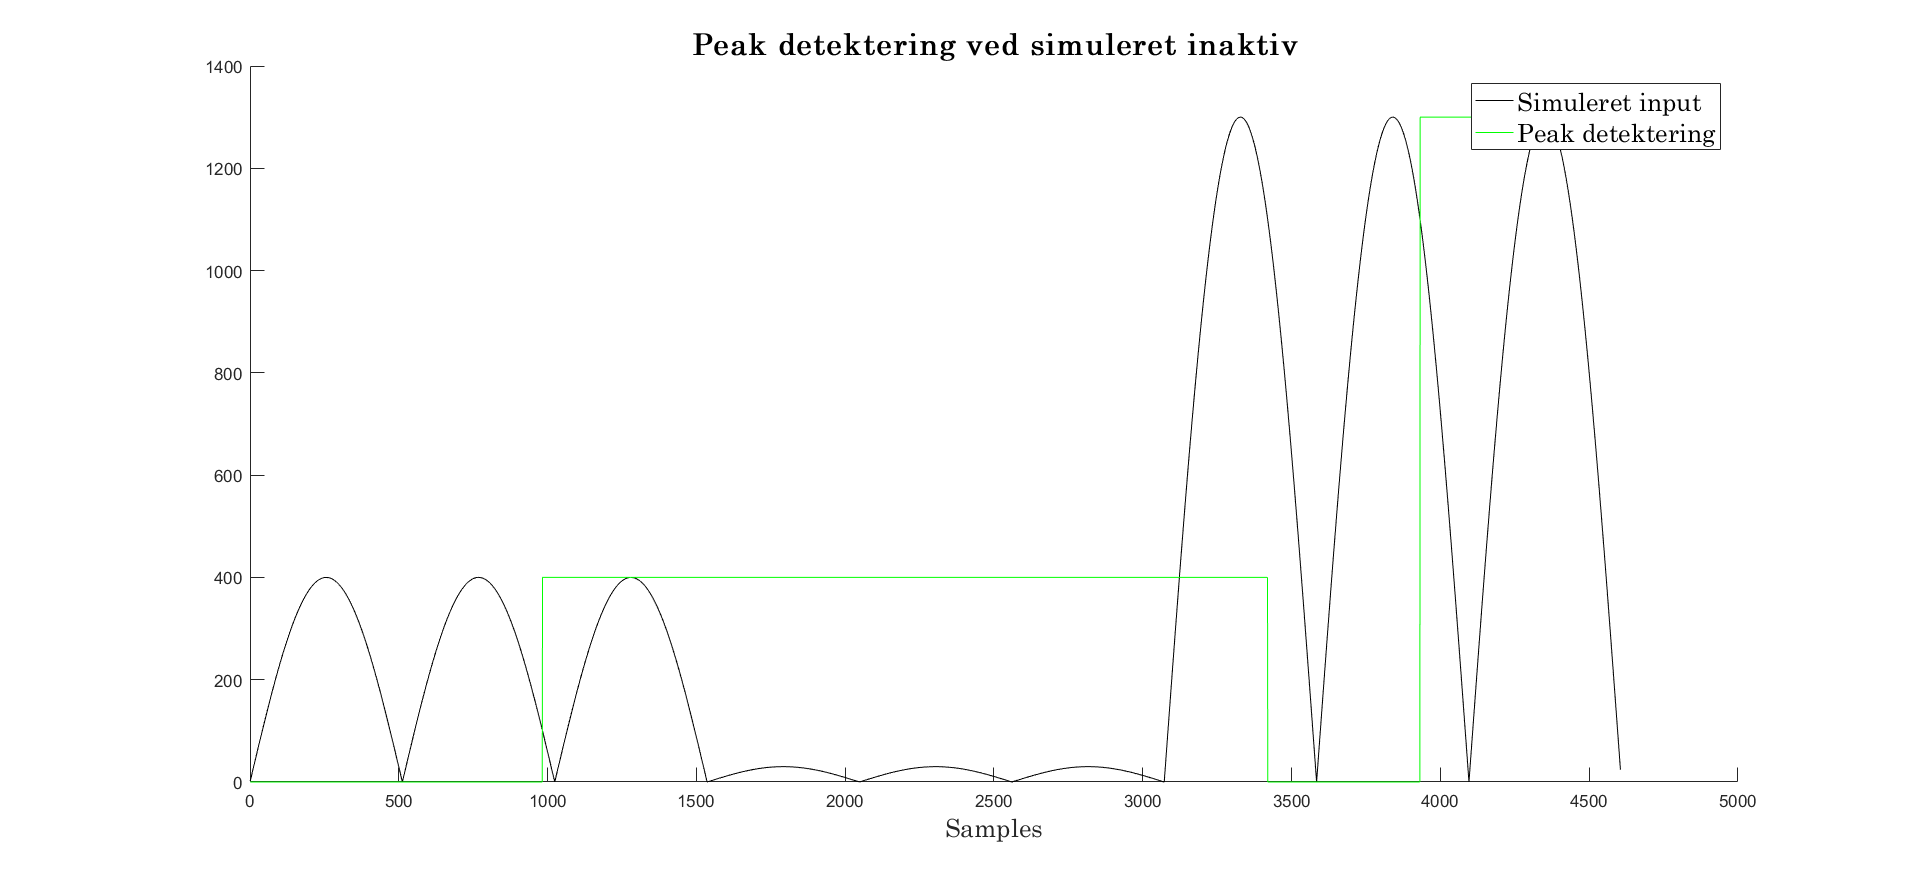
\includegraphics[width=.9\textwidth]{figures/cDesign/test_peak_inaktiv.png}
	\caption{På figuren ses algoritmens funktion til at detektere peakværdier, som resultat af detektering af et simuleret gang, inaktiv og løbe signal. Den sorte kurve er det simulerede signal, og den røde kurve er algoritmens funktion til detektering af peakværdier. }
	\label{fig:test_inaktiv_peak}
\end{figure}
Resultaterne vedrørende time count på \figref{fig:test_inaktiv_time} viser, at i perioden uden nogen aktivitet nulstilles time counteren ikke, før en sample har været over og under en tærskelværdi. Resultaterne vedrørende detektering af peak på \figref{fig:test_inaktiv_peak} viser, at første værdi tilhørende det første peak, samt det første peak efterfulgt fra ingen aktivitet frasorteres. For at klassificere hvorvidt algoritmen omhandlende detektering af ingen aktivitet fungerer efter hensigten, undersøges det data, der bliver videresendt som et resultat af perioder uden aktivitet. I tilfælde med et signalinput som ovenstående bør det første peak frasorteres efterfulgt af to værdier. Resultatet fra denne test fremgår i \tabref{tab:test_inaktiv}. %Derudover bør der registreres to time count værdier med tilhørende peakværdier efterfulgt af en periode med inaktivitet, hvoraf første peak frasorteres og dermed to time count værdier med tilhørende peak værdier.
\begin{table}[H]
	\centering
	\begin{tabular}{ccc}
		\hline
		\rowcolor[HTML]{C0C0C0} 
		Værdi videresendt & Forventet værdi & Modtaget værdi \\ \hline
		Time counter [samples] & $\emptyset$ - 512 - 512 - $\emptyset$ - 512 - 512 & $\emptyset$ - 512 - 512 - $\emptyset$ - 512 - 512 \\ \hline
		\multicolumn{1}{l}{Peak detektering [amplitude]} &     \multicolumn{1}{l}{$\emptyset$ - 200 - 200 - $\emptyset$ - 600 - 600}     &     \multicolumn{1}{l}{$\emptyset$ - 200 - 200 - $\emptyset$ - 600 - 600} \\ \hline
	\end{tabular}
	\caption{I tabellen ses testresultaterne vedrørende test af time count og detektering af peak ved et simuleret signal, som illustrerer en periode uden aktivitet. $\emptyset$ antyder at det ikke blev modtaget noget ved første peak. Der ses i tabellen, at algoritmen agerer efter hensigten.}
	\label{tab:test_inaktiv}
\end{table}\vspace{-0.5cm}
Algoritmen er blevet testet på et simuleret signal, som skulle illustrer en periode uden aktivitet omringet af to perioder med henholdsvis gang og løb. Det forventede resultat for både time count værdien og peakværdien er, at det første peak frasorteres, og første peak efter en periode uden aktivitet frasorteres. Dermed forventes det, at det videresendte data er time count på 512, og amplituder som afspejler signalets design på 200 og 600. Resultatet af det data, som blev modtaget, var som forventet med præcis nøjagtighed, og dermed kan det antages at algoritmens funktion vedrørende detektering af perioder uden aktivitet fungerer efter hensigten. Denne del af algoritmen accepteres og er klar til implementering i det samlede system.